\documentclass[10pt, aspectratio=169, usepdftitle=false]{beamer}

\usetheme[progressbar=frametitle]{metropolis}
\usepackage[danish]{babel}
\useoutertheme{infolines}
\setbeamertemplate{headline}{} % remove header

\usepackage{hyperref} %References
\hypersetup{
    pdftitle={SOP 2019 --- Præsentation},
    pdfauthor={Jens Tinggaard}
}

% meta info
\title{Studieområdeprojekt 2019}
\subtitle{Sikkerhed bag login-formular på en hjemmeside}
\date{27. januar 2020}
\author{Jens Tinggaard}
\institute{Odense Tekniske Gymnasium}
\titlegraphic{\hfill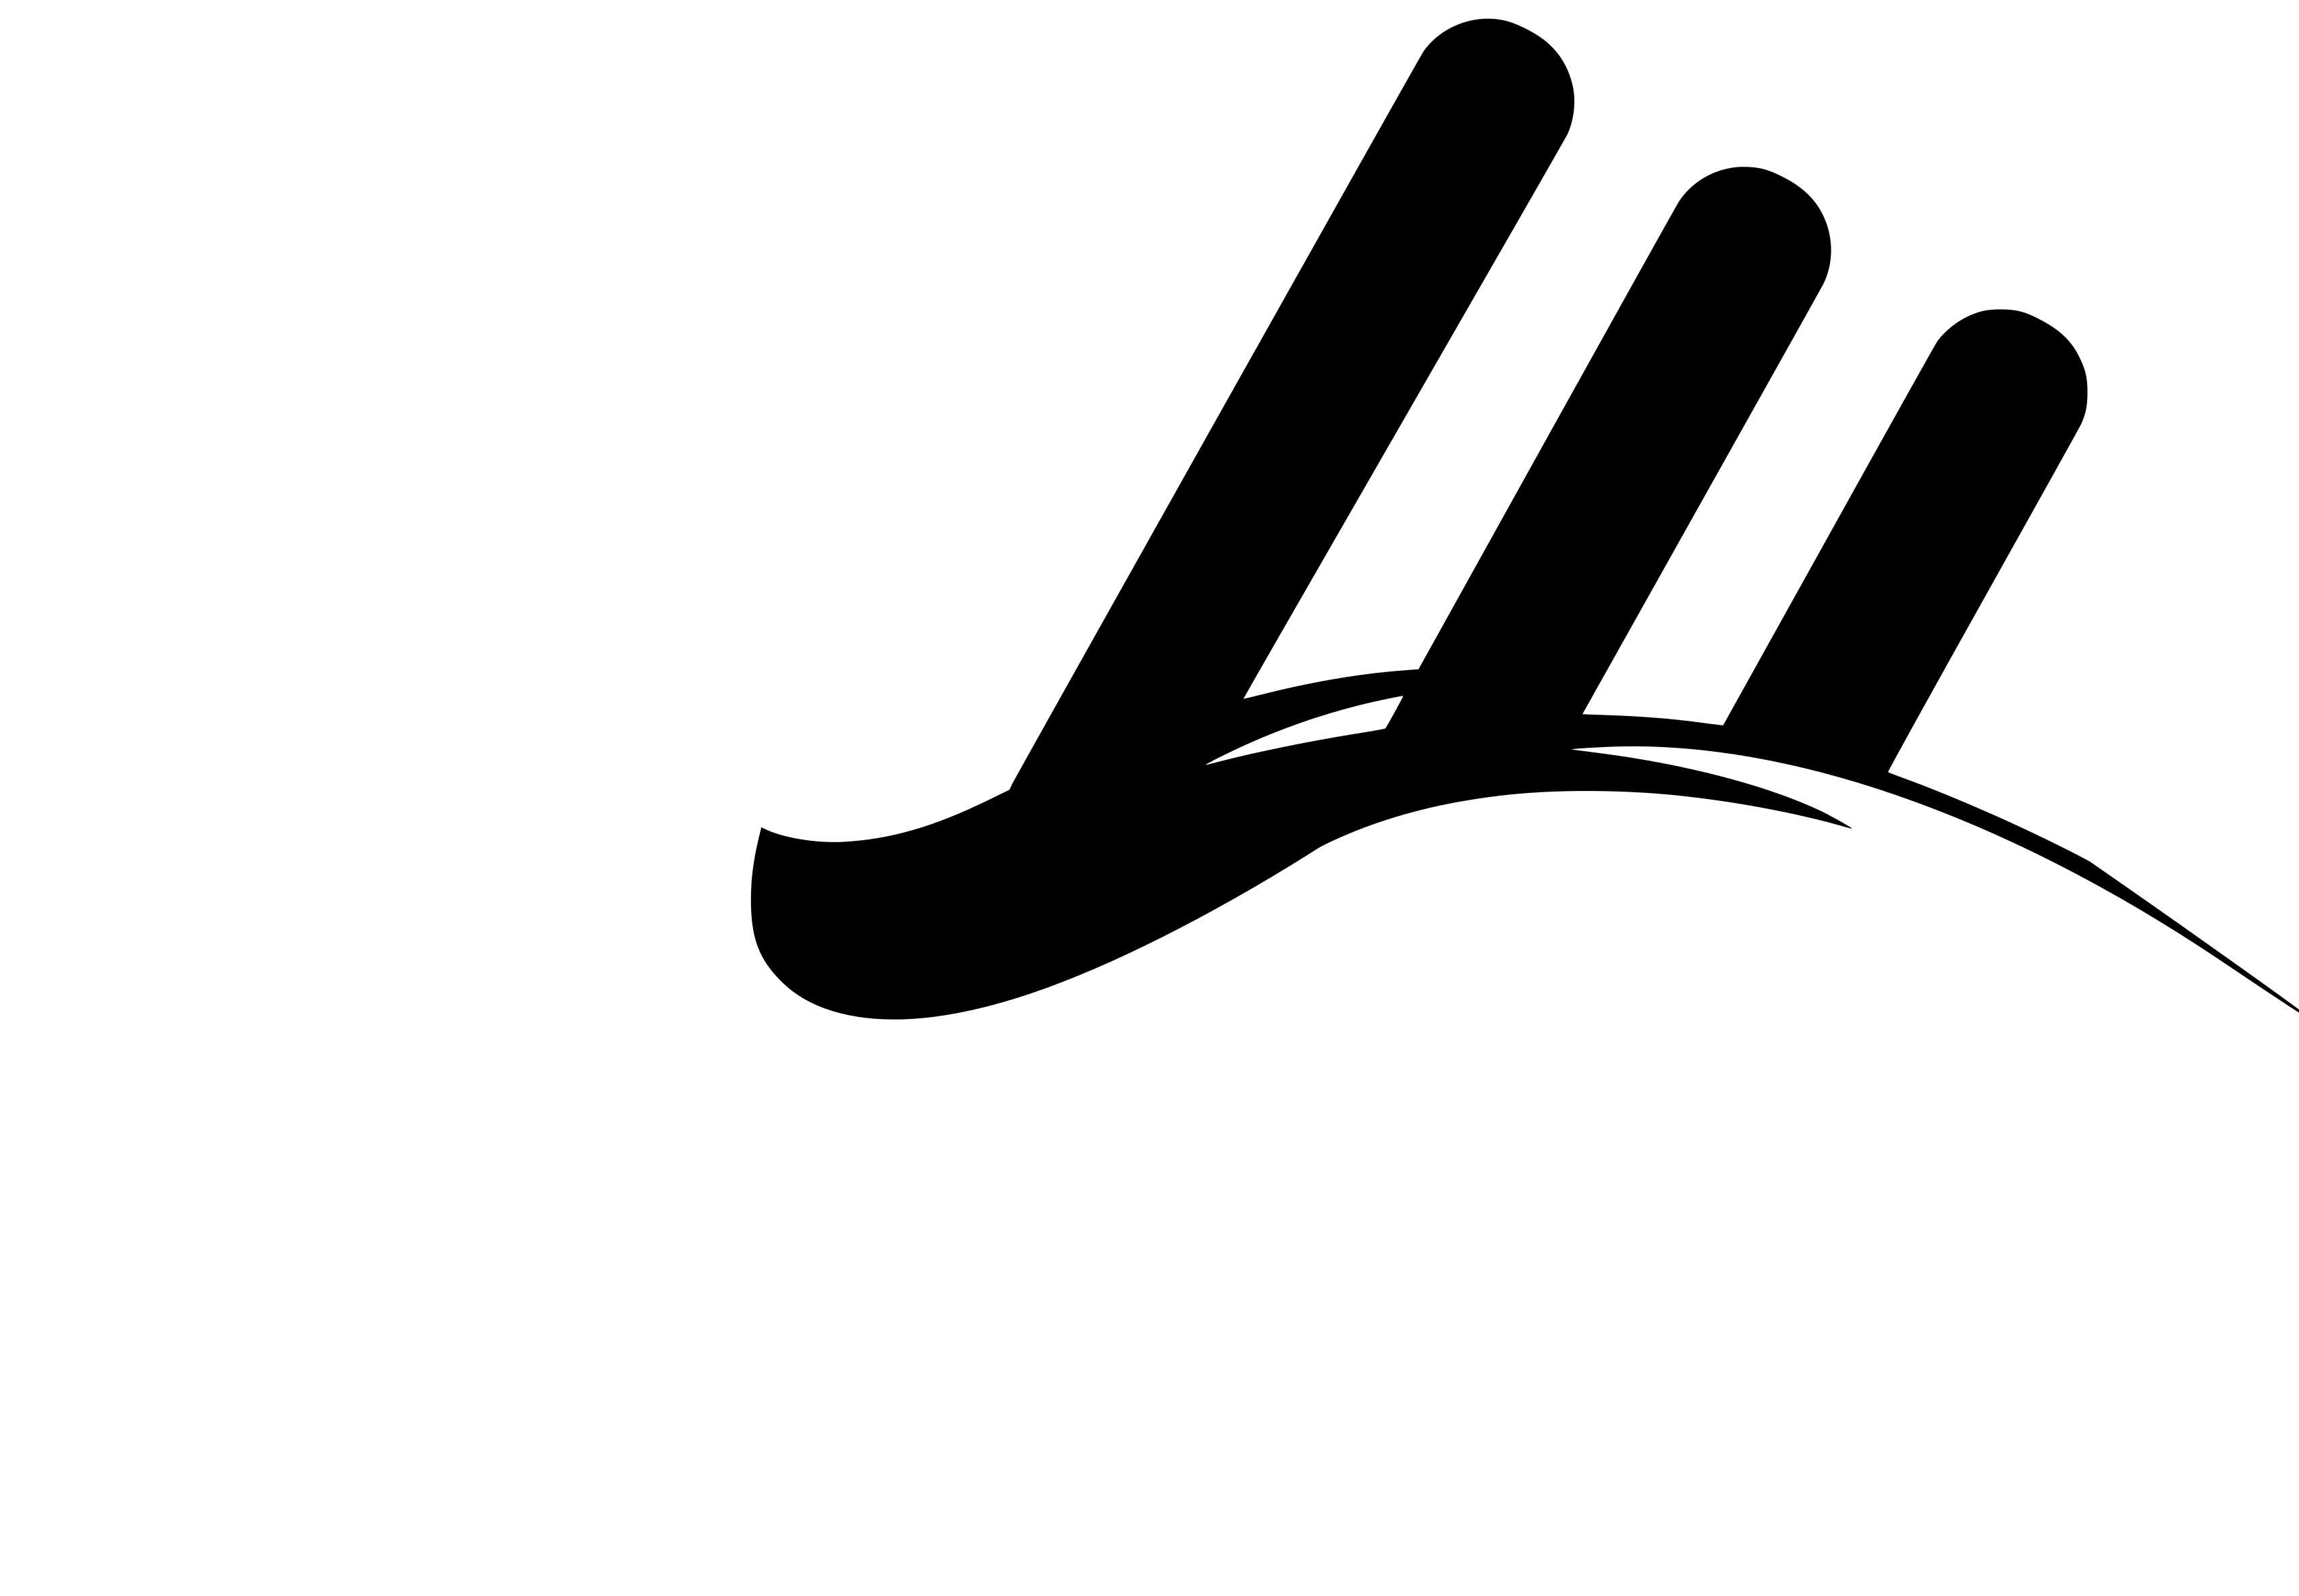
\includegraphics[height=1.5cm]{img/otg_logo.png}}


\begin{document}

\maketitle


\begin{frame}{Opgaveformulering}
    \large
    \begin{itemize}
        \item Redegør for talteorien bag RSA kryptering. Forklar nødvendigheden af primtal og hvordan RSA metoden fungerer.
        \item Gør kort rede for hashing.
        \item Analyser forskellen på hashing og kryptografi og hvilken rolle de har i forhold til sikkerhed.
        \item Vurder hvorfor RSA er vigtigt i forbindelse med sikkerhed ved logins.
    \end{itemize}
\end{frame}
%--- Next Frame ---%

\begin{frame}{Konklusion på projektet}
    \large
    \begin{itemize}
        \item Svært at primtalsfaktorisere et stort tal.
        \item Er essentielt for al onlinesikkerhed i dag.
        \item Metoder som RSA og hashing bliver sjældent brugt alene.
        \item Sikkerhedsfaktoere ved login.
    \end{itemize}
\end{frame}
%--- Next Frame ---%

\section{SOP som metodefag}
%--- Next Frame ---%

\begin{frame}{Relevante metoder i fagene}
    \large
    \begin{columns}[T,onlytextwidth]
        \column{0.5\textwidth}
            \alert{Matematik:}
            \begin{enumerate}
                \item Talteori.
                \item Deduktion \& ræsonnement.
                \item Analytiske løsninger.
                \item Eksempelføring.
            \end{enumerate}
        \column{0.5\textwidth}
            \alert{Programmering:}
            \begin{enumerate}
                \item Protokoller.
                \item Visualisering af id\'eer.
                \item Dokumentationslæsning.
            \end{enumerate}
    \end{columns}
\end{frame}
%--- Next Frame ---%


\begin{frame}{Empiri}
    \large
    \alert{Empiri brugt til udarbejdelse af projektet.}
    \begin{itemize}
        \item Dokumentation af programmer som \texttt{hashcat} og \texttt{gpg}.
        \item Standarder og protokoller til håndtering af disse.
        \item Virkelighedsdata.
    \end{itemize}
\end{frame}
%--- Next Frame ---%

\begin{frame}{Sammenspil mellem fagene}
    \large
    \alert{Tværfaglige metoder.}
    \begin{itemize}
        \item Logisk tankegang.
        \item Protokol \(\rightarrow\) matematisk fremgangsmåde.
        \item Anvendt matematik \(\rightarrow\) programmering.
    \end{itemize}
\end{frame}
%--- Next Frame ---%

\end{document}
